%
% main.tex -- Paper zum Thema fpga
%
% (c) 2019 Hochschule Rapperswil
%

%TODO IMPORTANT! CHange picture path to match buch.tex!!!!

\graphicspath{papers/fpga/}

\chapter{FPGA Implementation der schnellen Wavelet-Transformation\label{chapter:fpga}}
\lhead{FPGA Implementation der schnellen Wavelet-Transformation}
\begin{refsection}
\chapterauthor{Jonas Gründler und Nicolas Tobler}

\section{Introduction}
\rhead{Introduction}

VHDL, an acronym for Very High Speed Integrated Circuit Hardware Description Language is commonly used to implement fast, aplication-specific logic for an FPGA or custom silicon chip.
As every other programming language VHDL relies heavily on reuse of code.
Blocks of contained code can be stored as a semiconductor intellectual property core (IP core) and reused for further applications.
A often used IP core is the Fast Fourier Transform (FFT), which is available online for free.
Discrete wavelet transforms, however are not that common.
Therefore, we have committed ourselfs to implement a wavelet transform as a hardware block in VHDL

A hardware implemented wavelet algorithm has many advantages over a software implementation.
First, arithmetic operations in hardware are much faster than in software.
While a CPU is bond to its limited instruction set.
A custom hardware can execute multiple operations of choice in one clock cycle.
Some of operations can be executed in parallel in order to gain even more spped.
Secondly, if stream based processing is implemented, which continuously processes incoming data, the latency is significantly lower.
This property makes hardware superior for real time applications.

In the first part, this work covers the theory of an efficient algorithm for the discrete wavelet transform.
Then, the implementation of this algorithm in VHDL is described.

%Ready for deletion
%If you try to transform and modify audio signals, which are sampled with 44 kHz you get, because of the clock speed of the FPGA, which is about 100 MHz, over 1000 arithmetic operations for every audio sample.
%In the next few pages we guide through the theory used, some design considerations and at last through our steps of developing a basic but functional Wavelet Transformation in VHDL. 


\section{Discrete Wavelet Transform}
\rhead{Lifting Scheme}

The discrete wavelet transform (DTW) is covered in detail in chapter \ref{section:schnelle-synthese} of the script.
This section provides a short summary, as well as some additions, notably the Lifting Scheme.

The discrete wavelet transform is defined by a pair of formulas to calculate the wavelet coefficients $\bm a$ and $\bm b$.
$a_{j,k}$ and $b_{j,k}$ represent the coefficients in layer $j$ at the discrete time step $k$.
%The wavelet transform calculates $a_{j,k}$ and $b_{j,k}$ of layer $j$ from an input signal or coefficient $a_{j+1,k}$.
The formula to calculate the forward DTF is
\begin{align}
a_{j,k} = \sum_{l} \bar{h}_l a_{j+1,l+2k}
\\
b_{j,k} = \sum_{l} \bar{g}_l a_{j+1,l+2k} .
\end{align}
This calculation uses the Father and Mother wavelet coefficients $\bm{\bar h}$ and $\bm{\bar g}$, which are given from the chosen wavelet.
The inverse transform has been derived in the script as well: 
\begin{align}
a_{j+1,k} =
\sum_{l\in\mathbb Z}
h_{k-2l}
a_{j,l}
+
\sum_{l\in\mathbb Z}
g_{k-2l}
b_{j,l} .
\end{align}
%These formulas state the connection between two layers of a tower of wavelet transforms.
In order to create a connection between the theory covered in the script and additional theory, the z transform is used.
The z-transform of a FIR (finite impulse response) filter $h$ is a Laurent polynomial given by
\begin{equation}
h(z) = \sum_{k} h_k z^{-k}
\end{equation}
A convolution is equal to a multiplication in the z-domain.
The formulas from the script can be rewritten in the z-transform notation.
The forward transform becomes
\begin{align}
\quad a_{j,k}(z) &= \bar h(z^{-1}) a_{j+1,2k}(z) 
\\
\quad b_{j,k}(z) &= \bar g(z^{-1}) a_{j+1,2k}(z),
\end{align}
and the backward transform is
\begin{equation}
a_{j+1,k}(z) = h(z) a_{j,k}(z) + g(z) b_{j,k}(z).
\end{equation}
Figure \ref{fpga:fig:dwt} depicts a graphical representation of the DWT followed by an inverse DWT.
\begin{figure}
	\centering
	\usetikzlibrary{automata,arrows,positioning,calc}


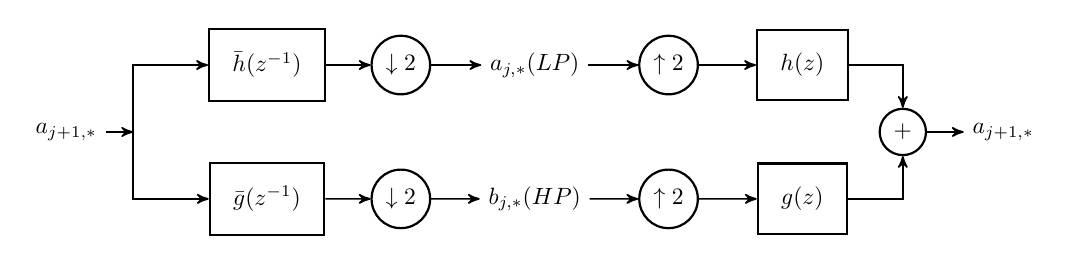
\begin{tikzpicture}[->, >=stealth', auto, semithick, node distance=2cm, scale = 0.85]

%\useasboundingbox (0,-0.5) rectangle (12.5,1.5);

\tikzstyle{every state}=[fill=white,draw=black,thick,text=black, scale = 1]
\tikzstyle{block}=[rectangle, inner sep=10pt, fill=white,draw=black,thick,text=black, scale = 1]
\tikzstyle{square}=[rectangle, fill=white,draw=black,thick,text=black, minimum height = 0.8cm, minimum width = 0.8cm, scale = 1]
\tikzstyle{round}=[circle, fill=white,draw=black,thick,text=black, scale = 1]
\tikzstyle{dots}=[fill=white,thick,text=black,scale=1]

\tikzset{every node/.style={scale=0.85}}
\tikzset{every coordinate/.style={scale=0.85}}

%\draw[step=1.0,black,thin,xshift=0.0cm,yshift=0.0cm] (-1,-3) grid (15,3);

\node[dots] (start) at (0,0) {$a_{j+1,*}$};

\coordinate     (split) at (1,0);

\node[block] (h1) at (3,1) {$\bar h(z^{-1})$};
\node[block] (h2) at (3,-1) {$\bar g(z^{-1})$};

\node[round] (d1) [right of=h1] {$\downarrow 2$};
\node[round] (d2) [right of=h2] {$\downarrow 2$};

\node[dots] (dots1) [right of=d1] {$a_{j,*} \- \text{(LP)}$};
\node[dots] (dots2) [right of=d2] {$b_{j,*} \- \text{(HP)}$};

\node[round] (u1) [right of=dots1] {$\uparrow 2$};
\node[round] (u2) [right of=dots2] {$\uparrow 2$};

\node[block] (hh1) [right of=u1] {$ h(z)$};
\node[block] (hh2) [right of=u2] {$ g(z)$};

\node[round] (combine) at (12.5,0) {$+$};

\node[dots, right of=combine, node distance=1.5cm] (end) {$a_{j+1,*}$} ;

\draw[->] (start) -- node {}(split);

\draw[->] (split) |- node {}(h1);
\draw[->] (split) |- node {}(h2);

\draw[->] (h1) -- node {}(d1);
\draw[->] (h2) -- node {}(d2);

\draw[->] (d1) -- node {}(dots1);
\draw[->] (d2) -- node {}(dots2);

\draw[->] (dots1) -- node {}(u1);
\draw[->] (dots2) -- node {}(u2);

\draw[->] (u1) -- node {}(hh1);
\draw[->] (u2) -- node {}(hh2);

\draw[->] (hh1) -| node {}(combine);
\draw[->] (hh2) -| node {}(combine);

\draw[->] (combine) -- node {}(end);

\end{tikzpicture}
	\caption{Discrete Wavelet transform and inverse transform}
	\label{fpga:fig:dwt}
\end{figure}

An input signal $\bm x$, where $x_k$ is its value at time step $k$, can be recursively transformed into a tower of wavelet coefficients.
$x_t$ is set equal to $a_{0,k}$ and represents the first layer of the tower.
This layer can be split into an arbitrarily long number of coefficients.
From all generated coefficients, only the $\bm b$ and the last layer of $\bm a$ coefficients are required, since they hold all information. %Dont like that sentence
Figure \ref{fpga:fig:dwtTower} shows a decomposition of 3 levels using DWTs and a subsequent unification using inverse DWTs.
\begin{figure}
	\centering
	\usetikzlibrary{automata,arrows,positioning,calc}

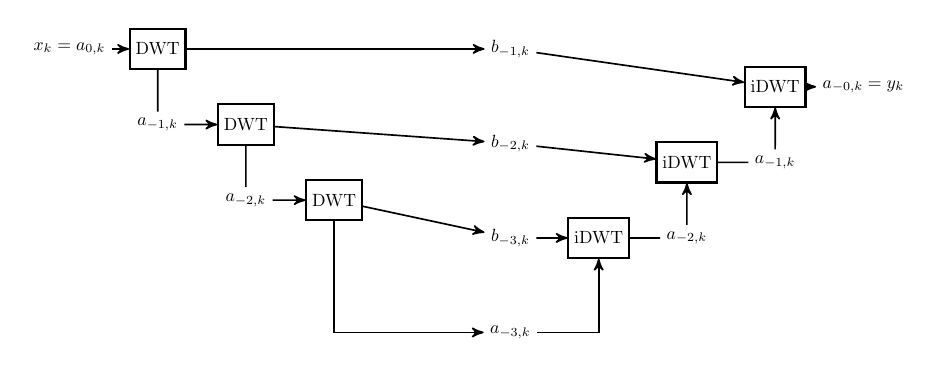
\begin{tikzpicture}[->, >=stealth', auto, semithick, node distance=1.5cm, scale = 0.8]

%\draw[step=1.0,black,thin,xshift=0.0cm,yshift=0.0cm] (-2,-8) grid (15,1);

%\useasboundingbox (0,-0.5) rectangle (12.5,1.5);

%\tikzset{every node/.style={scale=0.7}}

\tikzstyle{every state}=[fill=white,draw=black,thick,text=black,scale=0.8]
\tikzstyle{block}=[rectangle, inner sep=10pt, fill=white,draw=black,thick,text=black,scale=0.8]
\tikzstyle{square}=[rectangle, fill=white,draw=black,thick,text=black, minimum height = 0.8cm, minimum width = 0.8cm,scale=0.8]
\tikzstyle{round}=[circle, fill=white,draw=black,thick,text=black,scale=0.8]
\tikzstyle{dots}=[fill=white,thick,text=black,scale=0.8]

\node[dots] (a0) at (0,0) {$x_k = a_{0,k}$};

\node[square] (s1) [right of=a0, node distance=1.75cm] {DWT};
\node[dots] (b1) at (7 , 0) {$b_{-1,k}$};
\node[dots] (a1) [below of=s1] {$a_{-1,k}$};

\node[square] (s2) [right of=a1, node distance=1.75cm] {DWT};
\node[dots] (b2) at (7 , -1.5) {$b_{-2,k}$};
\node[dots] (a2) [below of=s2] {$a_{-2,k}$};

\node[square] (s3) [right of=a2, node distance=1.75cm] {DWT};
\node[dots] (b3) at (7 , -3) {$b_{-3,k}$};
\node[dots] (a3) at (7 , -4.5) {$a_{-3,k}$};

\node[square] (i3) [right of=b3, node distance=1.75cm] {iDWT};
\node[dots]   (ia3) [right of=i3, node distance=1.75cm] {$a_{-2,k}$};

\node[square] (i2) [above of=ia3] {iDWT};
\node[dots]   (ia2) [right of=i2, node distance=1.75cm] {$a_{-1,k}$};

\node[square] (i1) [above of=ia2] {iDWT};
\node[dots]   (ia1) [right of=i1, node distance=1.75cm] {$a_{-0,k} = y_k$};




\draw[->] (a0) -- (s1);
\draw[-] (s1) -- (a1);
\draw[->] (s1) -- (b1);


\draw[->] (a1) -- (s2);
\draw[-] (s2) -- (a2);
\draw[->] (s2) -- (b2);

\draw[->] (a2) -- (s3);
\draw[->] (s3) |- (a3);
\draw[->] (s3) -- (b3);

\draw[->] (a3) -| (i3);
\draw[->] (b3) -- (i3);
\draw[-] (i3) -- (ia3);

\draw[->] (ia3) -- (i2);
\draw[->] (b2) -- (i2);
\draw[-] (i2) -- (ia2);

\draw[->] (ia2) -- (i1);
\draw[->] (b1) -- (i1);
\draw[->] (i1) -- (ia1);



%
%\node[round] (d1) [right of=h1] {$\downarrow 2$};
%\node[round] (d2) [right of=h2] {$\downarrow 2$};
%
%\node[dots] (dots1) [right of=d1] {$a_{j,k} \- \text{(LP)}$};
%\node[dots] (dots2) [right of=d2] {$b_{j,k} \- \text{(HP)}$};
%
%\node[round] (u1) [right of=dots1] {$\uparrow 2$};
%\node[round] (u2) [right of=dots2] {$\uparrow 2$};
%
%\node[block] (hh1) [right of=u1] {$ h(z)$};
%\node[block] (hh2) [right of=u2] {$ g(z)$};
%
%\node[round] (combine) at (15,0) {$+$};
%
%\node[dots, right of=combine, node distance=1cm] (end) {$a_{j+1,k}$} ;

%\node[state]  (w1)          {$\omega_1$};
%
%\node[state]  (w0)    [left of=w1]                   {$\omega_0$};
%
%\node[state]  (w2)    [right of=w1]      {$\omega_2$};
%\node[dots]   (dotss) [right of=w2]      {...};
%\node[state]  (w5)    [right of=dotss]   {$\omega_5$};
%\node[state]  (w6)    [right of=w5]      {$\omega_6$};
%

c

%\draw[->] (split) |- node {}(h1);
%\draw[->] (split) |- node {}(h2);
%
%\draw[->] (h1) -- node {}(d1);
%\draw[->] (h2) -- node {}(d2);
%
%\draw[->] (d1) -- node {}(dots1);
%\draw[->] (d2) -- node {}(dots2);
%
%\draw[->] (dots1) -- node {}(u1);
%\draw[->] (dots2) -- node {}(u2);
%
%\draw[->] (u1) -- node {}(hh1);
%\draw[->] (u2) -- node {}(hh2);
%
%\draw[->] (hh1) -| node {}(combine);
%\draw[->] (hh2) -| node {}(combine);
%
%\draw[->] (combine) -- node {}(end);

%\path
%(start) edge[]       (split)
%     
%(split) edge[]     (w1);
%     
%(w1) edge[loop above]    node{$A_{1,1}$}     (w1)
%     edge[bend left]     node{$A_{1,2}$}     (w2)
%     
%(w2) edge[loop above]    node{$A_{2,2}$}     (w2)
%     edge[bend left]     node{$A_{2,3}$}     (dotss)
%
%(dotss) edge[bend left]    node{$A_{4,5}$}     (w5)
%     
%(w5) edge[loop above]    node{$A_{5,5}$}     (w5)
%     edge[bend left]     node{$A_{5,6}$}     (w6)
%     
%(w6) edge[loop above]    node{$A_{6,6}$}     (w6);


\end{tikzpicture}
	\caption{Tower of DWTs with 3 layers followed by a subsequent inverse transform tower.}
	\label{fpga:fig:dwtTower}
\end{figure}

%TODO Nic stopped here

\subsection{Lifting Scheme}
\rhead{Lifting Scheme}

The lifting scheme is a technique to perform a DWT efficiently.
It was introduced in a paper from Ingrid Daubechies and Wim Sveldens \cite{fpga:Daubechies1998}. 
The lifting scheme is an widely used algorithm, which is more efficient in terms of multiplication uses than normal wavelet transformations.
The number of arithmetic operations is reduced nearly by a factor of two compared to a ordinary, convolutional calculation.

The Lifting Scheme factorizes any discrete wavelet transform with finite filters into a series of elementary covolutions which are referred to as Lifting Steps.
This factorization splits a long filter into a tree of small filters, which is numerically superior in terms of rounding errors
This decomposition is equivalent to a factorization of the polyphase matrix of the wavelet filter into elementary matrices. 
In this paper, we want to focus only on orthogonal wavelets, where $\bm h = \bm{\bar h}$ and $\bm g = \bm{\bar g}$.
In order to be consistent with the paper, we use the semantics of Daubechies et al. which refer to the coefficients
\begin{align}
\bm a & \iff \bm s \quad \text{(smooth)} \quad \text{and} \\
\bm b & \iff \bm d \quad \text{(detail)} .
\end{align}

\subsubsection{Polyphase Decomposition \label{fpga:polyphase}}

The lifting scheme takes advantage of the polyphase decomposition.
The scaling relation leads to a downsampling factor of two.
This corresponds to splitting the signal into a channel for even samples $e$ and a channel for odd samples $o$.
The polyphase decomposition splits an algebraic expression into one part for each channel (polyphase components).
%The polyphase components are the filter components of the sub channels.
In order to continue in a polyphase implementation, all data, including the filter coefficients must be split as well.
This process is demonstrated with the $\bm h$ filter coefficients.
Its polyphase decomposition is
\begin{equation}
	h(z) = \sum_{n=-\infty}^{\infty} h_{2n} z^{-2n} + z^{-1} \sum_{n=-\infty}^{\infty} h_{2n+1} z^{-2n},
\end{equation}
or in the z-domain:
\begin{equation}
	h(z)=h_{e}(z^2) + z^{-1} h_o(z^2).
\end{equation}
This yields the even and odd components:
\begin{align}
	h_e(z) &= \sum_{n=-\infty}^{\infty} h_{2n}z^{-n}
	\\
	h_o(z) &= \sum_{n=-\infty}^{\infty} h_{2n+1}z^{-n}.
\end{align}

These coefficients are then placed together with the $g(z)$ components in the polyphase Matrix.
\begin{equation}
	\bm P(z) = 
	\begin{bmatrix}
	h_e(z) & g_e(z) \\
	h_o(z) & g_o(z)
	\end{bmatrix}
\end{equation}

Using the polyphase decomposition the DWT algorithm is
\begin{align}
\begin{bmatrix}
	s(z) \\
	d(z)
\end{bmatrix}
&=
\bm{\bar P}(z^{-1})^t
\begin{bmatrix}
	x(z^2) \\
	x(z^2) z
\end{bmatrix}
\\
\begin{bmatrix}
	y(z^2) \\
	y(z^2) z
\end{bmatrix}
&=
\bm P(z)
\begin{bmatrix}
	s(z) \\
	d(z)
\end{bmatrix}
,
\end{align}
where $x$ is the input of the forward DFT and $y$ is the reconstructed output of the inverse DFT.
The DFT using polyphase implementation is depicted graphically in figure \ref{fpga:fig:liftingSteps}.
\begin{figure}
	\centering
	%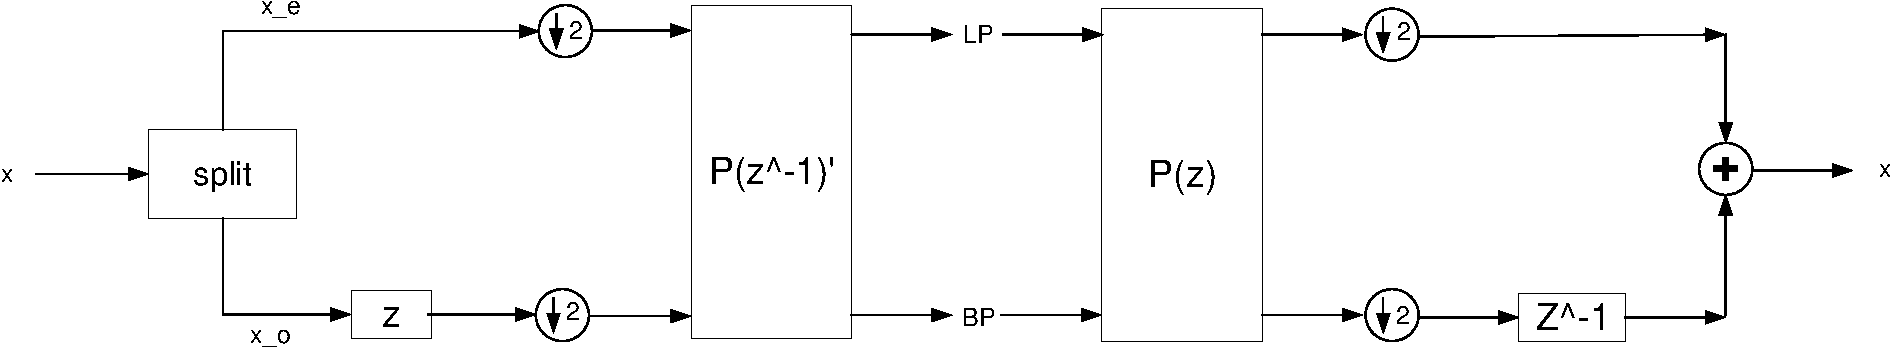
\includegraphics[width=\textwidth]{./images/lifting_step_wavelet.pdf}
	\usetikzlibrary{automata,arrows,positioning,calc}



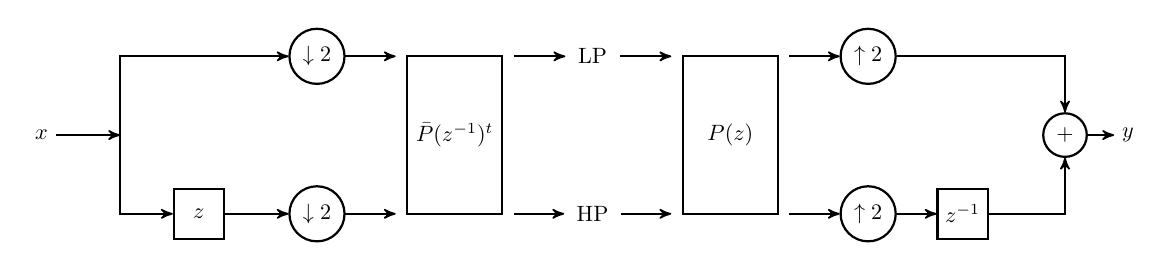
\begin{tikzpicture}[->, >=stealth', auto, semithick, node distance=1.5cm, scale = 1]


%\useasboundingbox (0,-0.5) rectangle (12.5,1.5);

%\tikzset{every node/.style={scale=0.7}}

\tikzstyle{block}=[rectangle, inner sep=4pt, fill=white,draw=black,thick,text=black, minimum height = 2.5cm, minimum width = 1.5cm, scale = 1]
\tikzstyle{square}=[rectangle, fill=white,draw=black,thick,text=black, minimum height = 0.8cm, minimum width = 0.8cm,  scale = 1]
\tikzstyle{round}=[circle, fill=white,draw=black,thick,text=black,  scale = 1]
\tikzstyle{dots}=[circle, fill=white,thick,text=black,scale=1, minimum size=0.8cm,  scale = 1]

%\draw[step=1.0,black,thin,xshift=0.0cm,yshift=0.0cm] (-2,-3) grid (10,3);

%\tikzset{every node/.style={scale=0.7}}

\node      (start) at(0,0) {$x$} ;

\coordinate (split)  at(1,0);

\node[] (z1)  {};
\node[square] (z2) at (2,-1) {$z$};

\node[round] (d1) at (3.5,1) {$\downarrow 2$};
\node[round] (d2) at (3.5,-1) {$\downarrow 2$};

\coordinate (h1tl) at (4.5, 1);
\coordinate (h1bl) at (4.5,-1);
\coordinate (h1tr) at (6, 1);
\coordinate (h1br) at (6,-1);
\node[block] (h1) at (5.25,0) {$\bm{\bar P}(z^{-1})^t$};



\node[dots] (dots1) at (7, 1) {\text{LP}};
\node[dots] (dots2) at (7, -1) {\text{HP}};

\coordinate (h2tl) at (8, 1);
\coordinate (h2bl) at (8,-1);
\coordinate (h2tr) at (9.5, 1);
\coordinate (h2br) at (9.5,-1);
\node[block] (h2) at (8.75,0) {$\bm P(z)$};


\node[round] (u1) at (10.5,1) {$\uparrow 2$};
\node[round] (u2) at (10.5,-1) {$\uparrow 2$};

\node[] (zz1) [right of=u1] {};
\node[square] (zz2) [right of=u2] {$z^{-1}$};

\node[round] (combine)  at (13,0){$+$};

\node[right of=combine, node distance=1cm] (end) {$y$};


\draw[->] (start) -- node {}(split);

\draw[->] (split) |- node {}(d1);
\draw[->] (split) |- node {}(z2);
\draw[->] (z2) -- node {}(d2);

\draw[->] (d1) -- node {}(h1tl);
\draw[->] (d2) -- node {}(h1bl);

\draw[->] (h1tr) -- node {}(dots1);
\draw[->] (h1br) -- node {}(dots2);

\draw[->] (dots1) -- node {}(h2tl);
\draw[->] (dots2) -- node {}(h2bl);

\draw[->] (h2tr) -- node {}(u1);
\draw[->] (h2br) -- node {}(u2);



\draw[->] (u1) -| node {}(combine);
\draw[->] (u2) -- node {}(zz2);
\draw[->] (zz2) -| node {}(combine);

\draw[->] (combine) -- node {}(end);


\end{tikzpicture}
	\caption{DWT graph using the polyface matrix $\bm P$}
	\label{fpga:fig:liftingSteps}
\end{figure}


\section{Lifting}

The core idea of the polyphase decomposition is the possibility of factorization of the $\bm P$ matrix.
Daubechies et al. proof, that this is possible for an arbitrary complementary matrix $\bm P$ if composed only of Laurent polynomials.
The factorization algorithm is of substantial length and is not explained in this work.
However, it results in the form
\begin{align}
	\bm{\bar P}(z) &=
	\Biggl(
	\prod_{i=1}^{m}
	\begin{bmatrix}
		1 & 0 \\
		-s_i(z^{-1}) & 1
	\end{bmatrix}
	\begin{bmatrix}
		1 & -t_i(z^{-1}) \\
		0 & 1
	\end{bmatrix}
	\Biggr)
	\begin{bmatrix}
		\frac{1}{K} & 0 \\
		0 & K
	\end{bmatrix}
	\\
	\bm P(z) &=
	\Biggl(
	\prod_{i=1}^{m}
	\begin{bmatrix}
		1 & s_i(z) \\
		0 & 1
	\end{bmatrix}
	\begin{bmatrix}
		1 & 0 \\
		t_i(z) & 1
	\end{bmatrix}
	\Biggr)
	\begin{bmatrix}
		K & 0 \\
		0 & \frac{1}{K}
	\end{bmatrix}
	.
\end{align}
Figure \ref{fpga:fig:liftingStepFactorization} shows a graphical version of the factorized DWT.
\begin{figure}
	\centering
	\usetikzlibrary{automata,arrows,positioning,calc}
\usetikzlibrary{shapes}

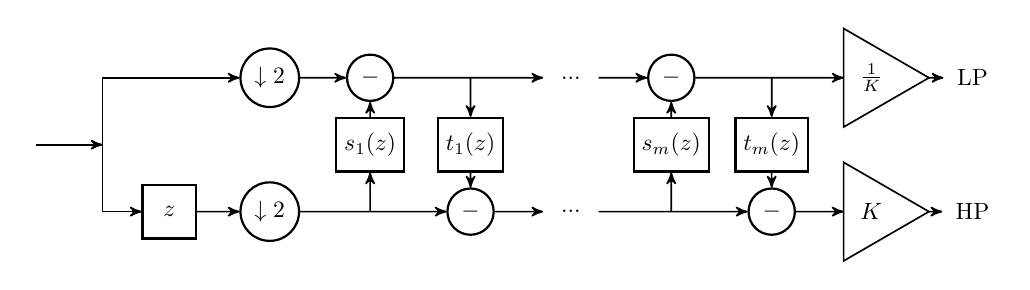
\begin{tikzpicture}[->, >=stealth', auto, semithick, node distance=1.5cm, scale = 0.85]

%\useasboundingbox (0,-0.5) rectangle (12.5,1.5);

\tikzstyle{block}=[rectangle, inner sep=4pt, fill=white,draw=black,thick,text=black, minimum height = 2.5cm, minimum width = 1.5cm, scale = 1]
\tikzstyle{square}=[rectangle, fill=white,draw=black,thick,text=black, minimum height = 0.8cm, minimum width = 0.8cm,  scale = 1]
\tikzstyle{round}=[circle, fill=white,draw=black,thick,text=black, scale = 1]
\tikzstyle{dots}=[circle, fill=white,thick,text=black, minimum size=0.8cm,  scale = 1]
\tikzstyle{amp}= [regular polygon, regular polygon sides=3,	draw, fill=white, text width=1em, inner sep=0.5mm, outer sep=0mm,	shape border rotate=-90, minimum size = 1.7cm, scale = 1]

\tikzset{every node/.style={scale=0.85}}
\tikzset{every coordinate/.style={scale=0.85}}

%\draw[step=1.0,black,thin,xshift=0.0cm,yshift=0.0cm] (-2,-3) grid (10,3);

\coordinate (start) at(0,0) ;

\coordinate (split)  at(1,0);

\node[] (z1)  {};
\node[square] (z2) at (2,-1) {$z$};

\node[round] (d1) at (3.5,1) {$\downarrow 2$};
\node[round] (d2) at (3.5,-1) {$\downarrow 2$};

\node[round] (min1) [right of=d1] {$-$};
\node[square] (s1) [below of=min1, node distance=1cm] {$s_1(z)$};
\coordinate[right of=d2] (c1) ;

\node[round] (min2) [right of=c1] {$-$};
\node[square] (s2) [above of=min2, node distance=1cm] {$t_1(z)$};
\coordinate[right of=min1] (c2) [right of=min1];

\node[dots] (dots1) [right of=c2] {...};
\node[dots] (dots2) [right of=min2] {...};

\node[round] (min3) [right of=dots1] {$-$};
\node[square] (s3) [below of=min3, node distance=1cm] {$s_m(z)$};
\coordinate[right of=dots2] (c3) ;

\node[round] (min4) [right of=c3] {$-$};
\node[square] (s4) [above of=min4, node distance=1cm] {$t_m(z)$};
\coordinate[right of=min3] (c4) [right of=min1];

\node[amp] (amp1) [right of=c4] {$\frac{1}{K}$};
\node[amp] (amp2)  [right of=min4] {$K$};

\node[dots] (lp) [right of=amp1] {\text{LP}};
\node[dots] (hp) [right of=amp2] {\text{HP}};


\draw[->] (start) -- (split);

\draw[->] (split) |- (d1);
\draw[->] (split) |- (z2);
\draw[->] (z2) -- (d2);


\draw[->] (d1) -- (min1);
\draw[->] (d2) -- (min2);

\draw[->] (c1) -- (s1);
\draw[->] (s1) -- (min1);
\draw[->] (c2) -- (s2);
\draw[->] (s2) -- (min2);

\draw[->] (min1) -- (dots1);
\draw[->] (min2) -- (dots2);


\draw[->] (dots1) -- (min3);
\draw[->] (dots2) -- (min4);

\draw[->] (c3) -- (s3);
\draw[->] (s3) -- (min3);
\draw[->] (c4) -- (s4);
\draw[->] (s4) -- (min4);

\draw[->] (min3) -- (amp1);
\draw[->] (min4) -- (amp2);

\draw[->] (amp1) -- (lp);
\draw[->] (amp2) -- (hp);

\end{tikzpicture}
	\usetikzlibrary{automata,arrows,positioning,calc}
\usetikzlibrary{shapes}

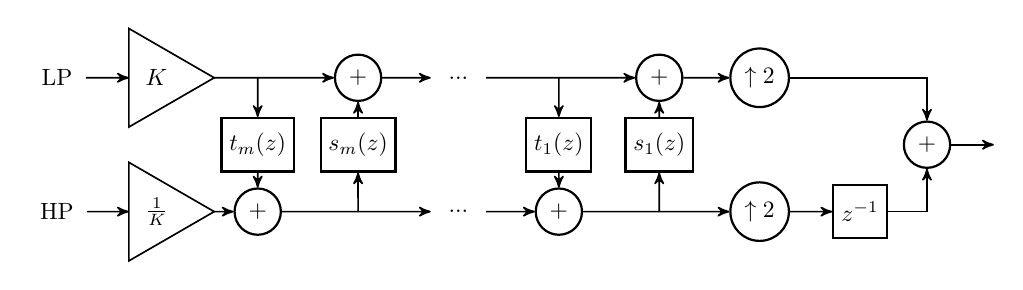
\begin{tikzpicture}[->, >=stealth', auto, semithick, node distance=1.5cm, scale = 0.85]

%\useasboundingbox (0,-0.5) rectangle (12.5,1.5);

\tikzstyle{block}=[rectangle, inner sep=4pt, fill=white,draw=black,thick,text=black, minimum height = 2.5cm, minimum width = 1.5cm, scale = 1]
\tikzstyle{square}=[rectangle, fill=white,draw=black,thick,text=black, minimum height = 0.8cm, minimum width = 0.8cm,  scale = 1]
\tikzstyle{round}=[circle, fill=white,draw=black,thick,text=black,  scale = 1]
\tikzstyle{dots}=[circle, fill=white,thick,text=black,scale=1, minimum size=0.8cm,  scale = 1]
\tikzstyle{amp}= [regular polygon, regular polygon sides=3,	draw, fill=white, text width=1em, inner sep=0.5mm, outer sep=0mm,	shape border rotate=-90, minimum size = 1.7cm, scale = 1]

\tikzset{every node/.style={scale=0.85}}
\tikzset{every coordinate/.style={scale=0.85}}

%\draw[step=1.0,black,thin,xshift=0.0cm,yshift=0.0cm] (-2,-3) grid (10,3);

\node[dots] (lp) at (0,1) {\text{LP}};
\node[dots] (hp) at (0,-1) {\text{HP}};

\node[amp] (amp1) [right of=lp] {$K$};
\node[amp] (amp2) [right of=hp] {$\frac{1}{K}$};


\coordinate[right of=amp1] (c1) ;
\node[round] (sum1) [right of=amp2] {$+$};
\node[square] (s1) [above of=sum1, node distance=1cm] {$t_m(z)$};

\coordinate[right of=sum1] (c2) ;
\node[round] (sum2) [right of=c1] {$+$};
\node[square] (s2) [below of=sum2, node distance=1cm] {$s_m(z)$};


\node[dots] (dots1) [right of=sum2] {...};
\node[dots] (dots2) [right of=c2] {...};


\coordinate[right of=dots1] (c3) ;
\node[round] (sum3) [right of=dots2] {$+$};
\node[square] (s3) [above of=sum3, node distance=1cm] {$t_1(z)$};

\coordinate[right of=sum3] (c4) ;
\node[round] (sum4) [right of=c3] {$+$};
\node[square] (s4) [below of=sum4, node distance=1cm] {$s_1(z)$};


\node[round] (u1) [right of=sum4] {$\uparrow 2$};
\node[round] (u2) [right of=c4] {$\uparrow 2$};

\node[square] (zz2) [right of=u2] {$z^{-1}$};

\node[round] (combine)  at (13,0){$+$};

\coordinate[right of=combine, node distance=1cm] (end);

\draw[->] (lp) -- (amp1);
\draw[->] (hp) -- (amp2);


\draw[->] (amp1) -- (sum2);
\draw[->] (amp2) -- (sum1);

\draw[->] (c1) -- (s1);
\draw[->] (s1) -- (sum1);
\draw[->] (c2) -- (s2);
\draw[->] (s2) -- (sum2);

\draw[->] (sum2) -- (dots1);
\draw[->] (sum1) -- (dots2);


\draw[->] (dots1) -- (sum4);
\draw[->] (dots2) -- (sum3);

\draw[->] (c3) -- (s3);
\draw[->] (s3) -- (sum3);
\draw[->] (c4) -- (s4);
\draw[->] (s4) -- (sum4);

\draw[->] (sum4) -- (u1);
\draw[->] (sum3) -- (u2);


\draw[->] (u1) -| (combine);
\draw[->] (u2) -- (zz2);
\draw[->] (zz2) -| (combine);

\draw[->] (combine) -- (end);

\end{tikzpicture}
	\caption{DWT signal flow graph with factorized filter functions (Lifting steps)}
	\label{fpga:fig:liftingStepFactorization}
\end{figure}
$\bm s(z)$ and $\bm t(z)$ result from the factorizing algorithm.
They replace $\bm h(z)$ and $\bm g(z)$ completely.



\subsection{Haar wavelet}
\label{fpga:sec:haar}

%Where $h_e(z)$ are the even- and $h_o(z)$ are the odd coefficients of the low pass filter.
%$g(z)$ is the corresponding high pass filter. 
For the sake of simplicity we initially chose the Haar Wavelet for the VHDL implementation, which constists of the following coefficients:
\begin{align}
h(z) = 1 + z^{-1} \quad & \Rightarrow \quad \bar h(z) = \frac{1}{2} + \frac{1}{2} z^{-1}
\\
g(z) = - \frac{1}{2} + \frac{1}{2} z^{-1} \quad & \Rightarrow \quad \bar g(z) = -1 + z^{-1}
\end{align}
If we split these coefficients into even and odd components and fill them into the polyphase matrix we get 

\begin{equation*}
\bm P(z) =
\begin{bmatrix}
1 & -\frac{1}{2} \\
1 & \frac{1}{2}
\end{bmatrix}
 = 
 \begin{bmatrix}
 1 & 0 \\
 1 & 1
 \end{bmatrix}
 \cdot
 \begin{bmatrix}
 1 & -\frac{1}{2} \\
 0 & 1
 \end{bmatrix}
\end{equation*}

The term on the right side is a possible factorization which results in lifting steps.
This factorizations produces diagonal matrices which are easy to compute and are the lifting steps.
This corresponds to the following implementation of the forward transform \cite{fpga:Daubechies1998}.
\begin{equation}\label{fpga:equation:haar}
	\begin{aligned}
	s_l^{(0)} &= x_{2l} \\
	d_l^{(0)} &= x_{2l+1} \\ 
	d_l &= d_l^{(0)} - s_l^{(0)} \\
	s_l &= s_l^{(0)} + \frac{1}{2}d_l
	\end{aligned}
\end{equation}
where $x_{n}$ is the incoming sample stream.
The analysis side is in the following form:
\begin{equation*}
\bm {\bar P}(z^{-1})^t =
\begin{bmatrix}
\frac{1}{2} & \frac{1}{2} \\
-1 & 1
\end{bmatrix}
= 
\begin{bmatrix}
1 & \frac{1}{2} \\
0 & 1
\end{bmatrix}
\cdot
\begin{bmatrix}
1 & 0 \\
-1 & 1
\end{bmatrix}
\end{equation*}
In this case the inverse transformation is 
\begin{equation}\label{fpga:equation:inv_haar}
\begin{aligned}
s_l^{(0)} &= s_l - \frac{1}{2}d_l \\
d_l^{(0)} &= d_l + s_l \\ 
x_{2l+1}& =d_l^{(0)} \\
x_{2l} &= s_l^{(0)}
\end{aligned}
\end{equation}
and the original stream can be fully recovered.
Figure \ref{fpga:fig:liftingStepHaar} shoes both transforms graphically.
\begin{figure}
	\centering
	\usetikzlibrary{automata,arrows,positioning,calc}
\usetikzlibrary{shapes}


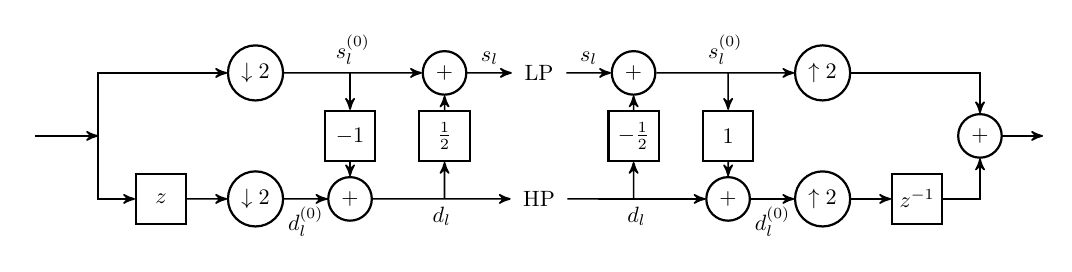
\begin{tikzpicture}[->, >=stealth', auto, semithick, node distance=1.5cm, scale = 0.8]


%\useasboundingbox (0,-0.5) rectangle (12.5,1.5);



\tikzstyle{block}=[rectangle, inner sep=4pt, fill=white,draw=black,thick,text=black, minimum height = 2.5cm, minimum width = 1.5cm, scale = 1]
\tikzstyle{square}=[rectangle, fill=white,draw=black,thick,text=black, minimum height = 0.8cm, minimum width = 0.8cm,  scale = 1]
\tikzstyle{round}=[circle, fill=white,draw=black,thick,text=black,  scale = 1]

\tikzstyle{dots}=[circle, fill=white,thick,text=black,scale=1, minimum size=0.8cm,  scale = 1]

\tikzstyle{amp}= [regular polygon, regular polygon sides=3,	draw, fill=white, text width=1em, inner sep=0.5mm, outer sep=0mm, shape border rotate=-90, minimum size = 1.7cm, scale = 1]

\tikzset{every node/.style={scale=0.8}}
\tikzset{every coordinate/.style={scale=0.8}}

%\draw[step=1.0,black,thin,xshift=0.0cm,yshift=0.0cm] (-2,-3) grid (10,3);

%\tikzset{every node/.style={scale=0.7}}

\coordinate      (start) at(0,0) ;

\coordinate (split)  at(1,0);

\node[] (z1)  {};
\node[square] (z2) at (2,-1) {$z$};

\node[round] (d1) at (3.5,1) {$\downarrow 2$};
\node[round] (d2) at (3.5,-1) {$\downarrow 2$};



\node[round] (sum1) [right of=d2] {$+$};
\node[square] (s1) [above of=sum1, node distance=1cm] {$-1$};
\coordinate[right of=d1] (c1);

\node[round] (sum2) [right of=c1] {$+$};
\node[square] (s2) [below of=sum2, node distance=1cm] {$\frac{1}{2}$};
\coordinate[right of=sum1] (c2) ;

\node[dots] (hp) [right of=sum2] {\text{LP}};
\node[dots] (lp) [right of=c2]   {\text{HP}};



\coordinate[right of=lp] (c3);
\node[round] (sum3) [right of=hp] {$+$};
\node[square] (s3) [below of=sum3, node distance=1cm] {$-\frac{1}{2}$};

\coordinate[right of=sum3] (c4) ;
\node[round] (sum4) [right of=c3] {$+$};
\node[square] (s4) [above of=sum4, node distance=1cm] {$1$};


\node[round] (u1) [right of=c4] {$\uparrow 2$};
\node[round] (u2) [right of=sum4] {$\uparrow 2$};

\node[square] (zz2) [right of=u2] {$z^{-1}$};

\node[round] (combine)  at (15,0){$+$};

\coordinate[right of=combine, node distance=1cm] (end);


\draw[->] (start) -- (split);

\draw[->] (split) |- (d1);
\draw[->] (split) |- (z2);
\draw[->] (z2) -- (d2);


\draw[->] (d1) -- node[above]{$s_l^{(0)}$} (sum2);
\draw[->] (d2) -- node[below]{$d_l^{(0)}$} (sum1);

\draw[->] (c1) -- (s1);
\draw[->] (s1) -- (sum1);
\draw[->] (c2) -- (s2);
\draw[->] (s2) -- (sum2);

\draw[->] (sum2) -- node[above]{$s_l$} (hp);
\draw[->] (sum1) -- node[below]{$d_l$} (lp);

\draw[->] (hp) -- node[above]{$s_l$} (sum3);
\draw[->] (lp) -- node[below]{$d_l$} (sum4);



\draw[->] (c3) -- (s3);
\draw[->] (s3) -- (sum3);
\draw[->] (c4) -- (s4);
\draw[->] (s4) -- (sum4);

\draw[->] (sum3) -- node[above]{$s_l^{(0)}$}(u1);
\draw[->] (sum4) -- node[below]{$d_l^{(0)}$}(u2);


\draw[->] (u1) -| (combine);
\draw[->] (u2) -- (zz2);
\draw[->] (zz2) -| (combine);

\draw[->] (combine) -- (end);


\end{tikzpicture}
	\caption{Lifting scheme implementation of the Haar wavelet.}
	\label{fpga:fig:liftingStepHaar}
\end{figure}

\section{VHDL Implementation}

The VHDL implementation adds some complexity to the mathematical representation of the algorithm.
A physical implementation allows only causal filters.
These are recognizable by containing solely negative exponentials of $z$.
All non-causal filters must be delayed, in order to get causal.
Notably, the polyface decomposition of the forward wavelet transform is non-causal and must be delayed by one sample.

\subsection{Design Considerations}

When implementing an algorithm in hardware, a lot of design considerations must be made in advance.
The hardware architecture is very dependent of the application.
A hardware block can be optimized for various points, such as high accuracy, low latency, high data rate, low area and low power consumption.
Since this work is not based on a defined objective, we must come up with our own design specifications.

In most cases, which do not require low latency and high data rates, a digital signal processor would be a better choice than a custom VHDL-implemented hardware.
A sequential processor unit is computationally very efficient and requires almost no area compared to most VHDL solutions.
However, it features a significantly higher latency, which is a major drawback.
Hence, the VHDL implementation should feature low latency and high data rate as its main objectives in order to provide solution, that is reasonable as a hardware implementation.
The application should make use of on of the biggest advantages of custom hardware, which is parallelism.
Performing calculations in parallel leads to higher throughput and allows data rates which are as fast as the clock speed of the logic.
The strengths of the aspired implementation are thus high speed and low latency processing, suitable for real-time applications.

The main priority is to implement the Haar wavelet.
A optional goal is the implementation of a higher order wavelet, such as the orthogonal Daubechies-4 wavelet.
The implementation should be as generic as possible, in order to allow customization.

\subsection{Idea}

A forward and inverse multiresolution analysis DFT should be implemented, where each function is contained in a VHDL entity.
Figure \ref{fpga:fig:idea} shows the outline of the two blocks.
\begin{figure}
	\centering
	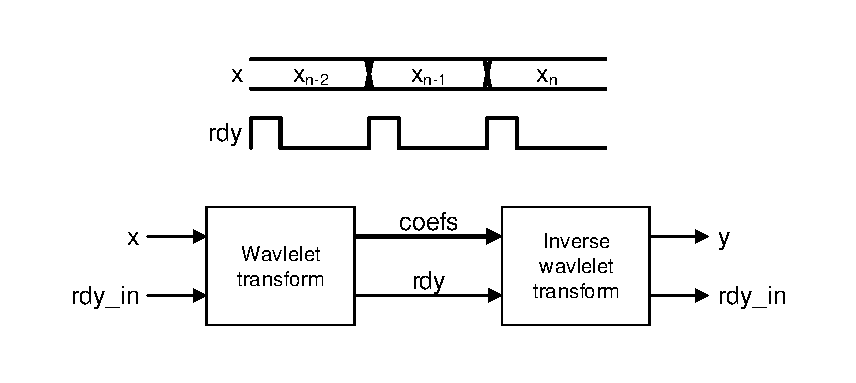
\includegraphics[width=0.8\textwidth]{papers/fpga/images/idea.pdf}
	\caption{Outline of the modules \label{fpga:fig:idea}}
\end{figure}
The number of multiresolution layers \texttt{N} can be specified as a generic parameter.
The forward algorithm has a 16-bit signed number input \texttt{x} ($a_{j,k} \forall k=0$) and outputs the wavelet coefficients as a stream.
Each signal is accompanied by a ready signal which is driven \texttt{1} if the coefficient has been newly calculated.
If this ready signal is always driven high, the input value is sampled each clock cycle.
The coefficients are in form of a vector \texttt{d\_s}, which holds \texttt{N} detail coefficients ($b_{j,k} \forall k \in [-1 .. -N]$) and \texttt{s}, which holds remaining smooth coefficient ($a_{j,k} \forall k=-N$).
The coefficients are accompanied by a vector of ready signals with length \texttt{N}, where each element corresponds to a level of the multiresolution analysis.
The inverse block has the coefficients and ready signals as input and outputs the reconstructed signal \texttt{y}, again accompanied by its ready signal.

\subsection{Architecture}
The following sections describe the internal blocks in detail.


\subsubsection{Forward and backward transformation}

It takes a 16-bit number as its input which is processed when the associated ready signal is driven high.
The outputs consist of an array of wavelet coefficients, each of 16 bits, which are accompanied with a vector of ready signals. 

The inverse wavelet transform \texttt{inv\_haar} has an analogous outline.
The blocks are fed with the different coefficients and they get processed by the algorithm defined in equation \ref{fpga:equation:inv_haar}.
In this process the input coefficients are reconstructed to a 16-bit signed output number.
% in the \texttt{inv\_branching} block, which holds several blocks of inverse wavelet transforms.

%TODO make figure of delay

\subsubsection{Wavelet transform}

The transformation block \texttt{haar} implements the algorithm needed for the wavelet transformation.
So far, only the Haar wavelets has been implemented.
However, the outline stays the same for every other discrete wavelet.
Figure \ref{fpga:fig:haar} shows the outlihne of the \texttt{haar} and \texttt{inv\_haar} block.
\begin{figure}
	\centering
	\includegraphics[width=0.49\textwidth]{papers/fpga/images/haar.pdf} %TODO fix rdy signal
	\includegraphics[width=0.49\textwidth]{papers/fpga/images/inv_haar.pdf}
	\caption{Complete architecture \label{fpga:fig:haar}}
\end{figure}
The output of the \texttt{haar} block features the half sample rate due to the down sampling operator.
The forward transform, which is in mathematical notation non-causal, has been delayed in order to be causal.
In order to contain the propagation delay, a flip-flop is inserted at the end of the block.
This leads to another delay of one clock cycle.
The arithmetic inside the blocks are implemented as derived in section \ref{fpga:sec:haar}.
In the case of the Haar wavelet, the arithmetic is a fairly simple sequence of calculations as  described in equation \ref{fpga:equation:haar}.
Multiplications and divisions with the number 2 can efficiently be implemented with a bit shift.

%Because of the generalized structure and of VHDL in general this blocks can be adapted to different algorithms to perform transformations with different wavelets.

\subsubsection{Multiresolution analysis}

The multiresolution analysis is achieved by chaining the wavelet transform blocks.
The block which holds the multiresolution analysis is called \texttt{branching}.
Hereby, the lowpass output (\texttt{s}) of each DFT block (\texttt{haar}) is connected to the input of annother DFT block, which performs another transformation to increase detail. 

%Insert graph of vhdl simulation 

So the upper mentioned process contains multiple wavelet-blocks which together perform a multiresolution analysis.
Since each layer splits a input data stream in half, this block is called \texttt{braching}.
The Lowpass output ($s$) samples of a Haar block are connected to another Haar block 
Because of this we need the also delayed ready signal from the last block because these coefficients are changing with half of the speed now. 
The inverse branching is then used to reconstruct the original signal from all the different transformations and coefficients.


\subsubsection{Delay}

The \texttt{branching} and \texttt{inv\_branching} block are sufficient for the objective. %dont like that

However the output of the forward transform and the input of the inverse transform are not compatible
In order to make them connectable, a delay block must be inserted in between of the two blocks.
Figure \ref{fpga:fig:mainDelay} shows the connected blocks.
In this formation the input \texttt{x} is converted to wavelet coefficients and subsequently reconstructed to the output \texttt{y}.
\texttt{y} should be equal to the signal \texttt{x}, if delayed with the latency of the blocks, considering numerical accuracy
\begin{figure}
	\centering
	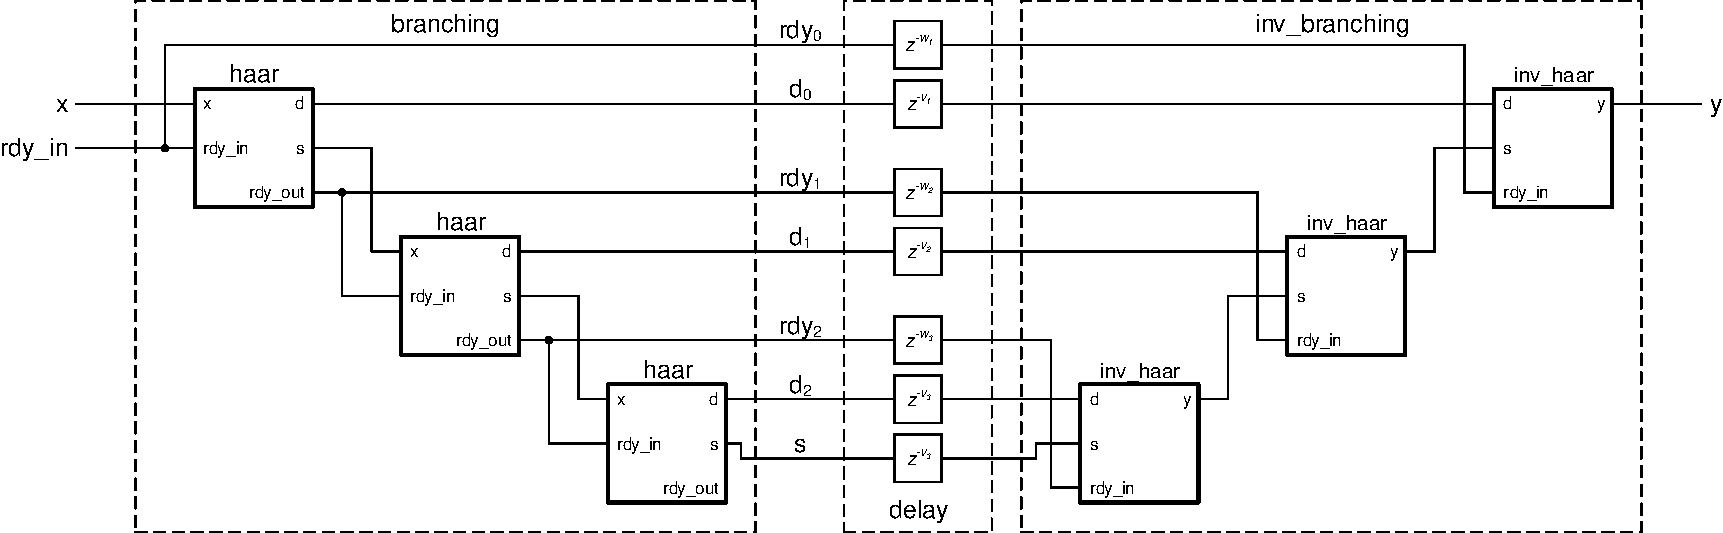
\includegraphics[width=\textwidth]{papers/fpga/images/main_delay.pdf}
	\caption{Complete architecture \label{fpga:fig:mainDelay}}
\end{figure}


%TODO rewrite this block
In order to provide low-latency regardless, a compromise has been made, which tolerates a delay of one cyle in each layer of the muliresolution analysis.
Because of this one clock cycle of delay in the transformation block the faster coefficients need to be artificially delayed.
If not they arrive to early at the inverse transformation and the result is faulty. To compensate this the   faster signals get delayed according to de depth of the recursion tree.
The coefficients containing the lowest frequencies stay the same and then for every step up on the recursion tree the delay gets one clock cycle longer.
With this processing the coefficients with belong together arrive at the inverse transformation at the same time.

All coefficients except the one with the lowest frequency must be delayed for the inverse algorithm.


\subsection{Testing}

The test structure contains the forward transform, followed by the inverse transform, which should recover the original signal from the processed coefficients.
The depth of the branching and the recursion can be set by a variable. 
The test setup is shown in figure \ref{fpga:fig:testing}
If done right, the output should resemble the input, delayed by the latency of the whole pipeline.

\begin{figure}
	\centering
	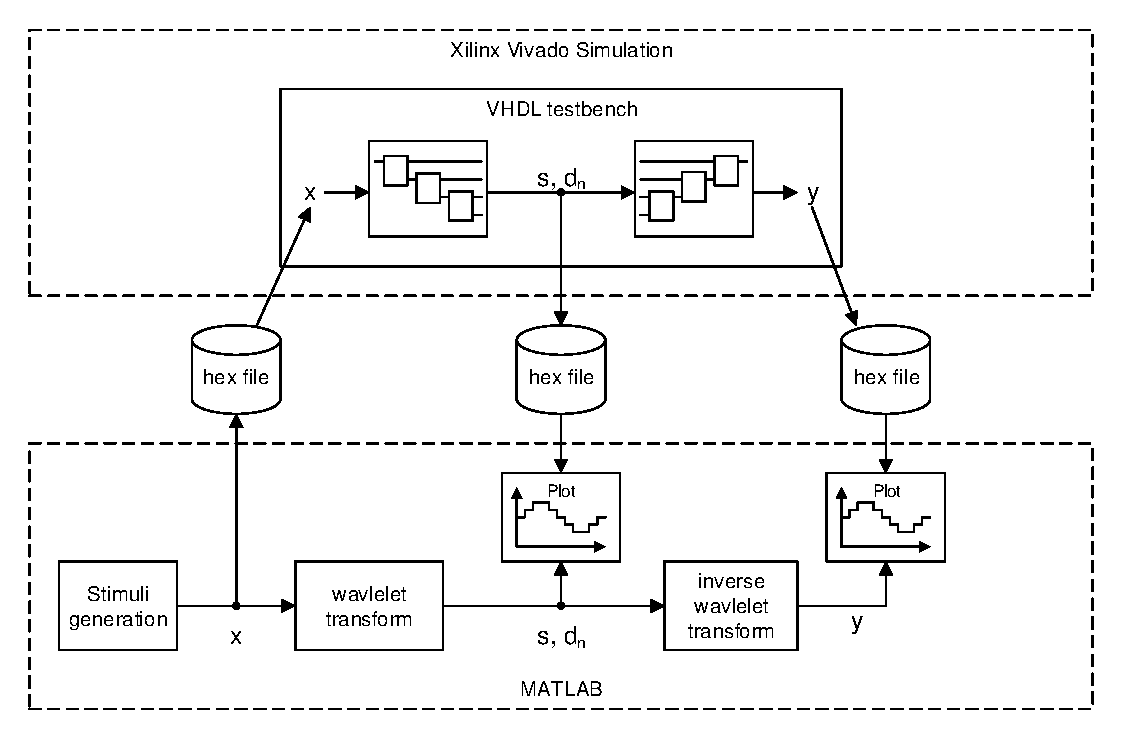
\includegraphics[width=\textwidth]{papers/fpga/images/vhdl_sim.pdf}
	\caption{Testing Workflow \label{fpga:fig:testing}}
\end{figure}

The Vivado Toolchain from Xilix has been used to simulate the VHDL modules.
The wavelet transforms have also been implemented numerically identical in MATLAB in order to provide a direct comparison. 
A set of helper modules have been implemented in VHDL 2008, which are able to read and write test vectors and results from or to a file.
These modules provide an an easy way to inject test data from the MATLAB enviroment.
After the VHDL simulation finishes, the results are again fed into MATLAB for validation.

\section{Results}
\rhead{Results}

The results are promising. The results of the Vivado Toolchain and MATLAB match up. 
In picture \ref{fpga:fig:coeff} the coefficients and ready signals before delaying are depicted.
The delay of the ready signals, stepping into the recursion tree, gets doubled every step. 
And the wavelet coefficients are also plotted in different colors. 
The faster changing signals correspond to the higher frequencies and the slow changing signals are deeper in the recursion.
The higher frequencies also react faster to changes at the input.
\begin{figure}
	\centering
	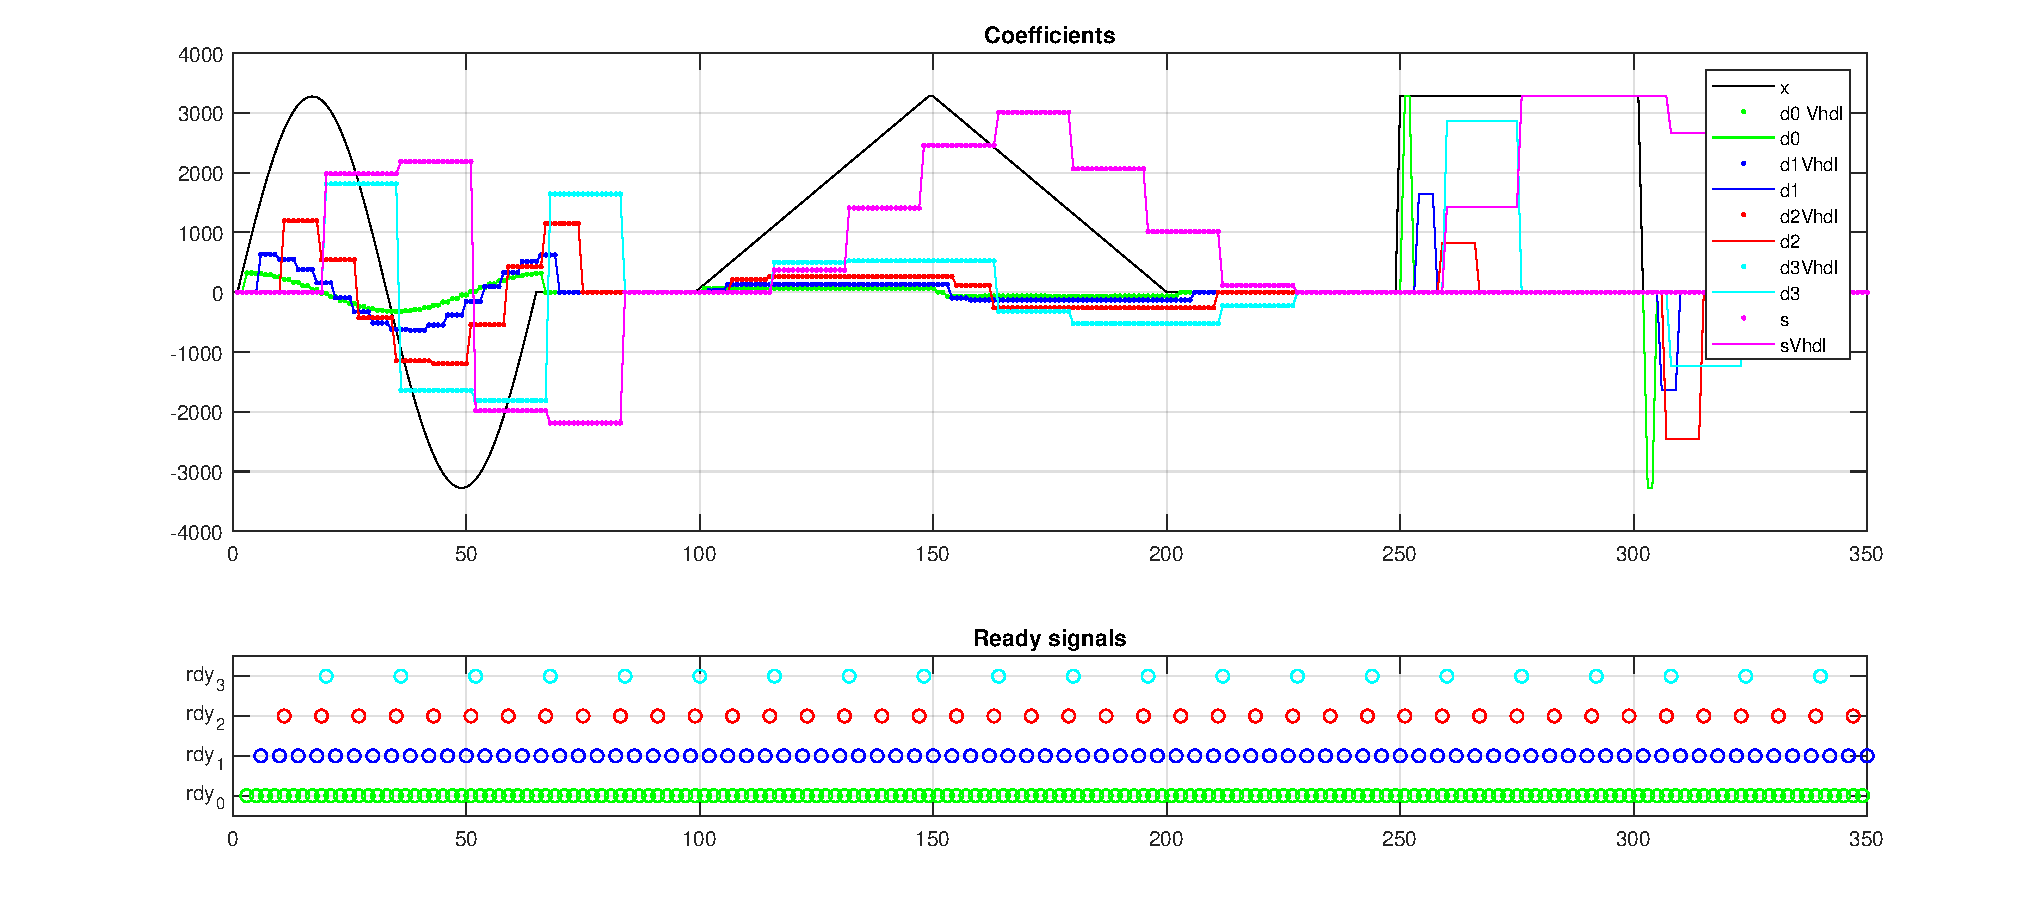
\includegraphics[width=\textwidth]{papers/fpga/images/coefs.pdf}
	\caption{Coefficients and ready signals after transformation \label{fpga:fig:coeff}}
\end{figure}

Picture \ref{fpga:fig:coeff_delayed} shows the coefficients and ready signals after delaying. 
As visible the coefficients start to change now delayed only by clock cycle. 
Like this there is no misalignment in the time domain and when they are transformed back the original signal is recovered. 
The ready signal illustrates this. 
Before the delaying the ready signal of the fast coefficients was first and the slower ones where delayed. 
But in reality the slower frequencies change at the same moment as the higher frequencies. 
And also the information from the high frequencies is also needed at the moment when the inverse transformation starts. 
So after the delaying the slow ready signal arrives first and then with every clock cycle the faster readys arrive. 
\begin{figure}[h]
	\centering
	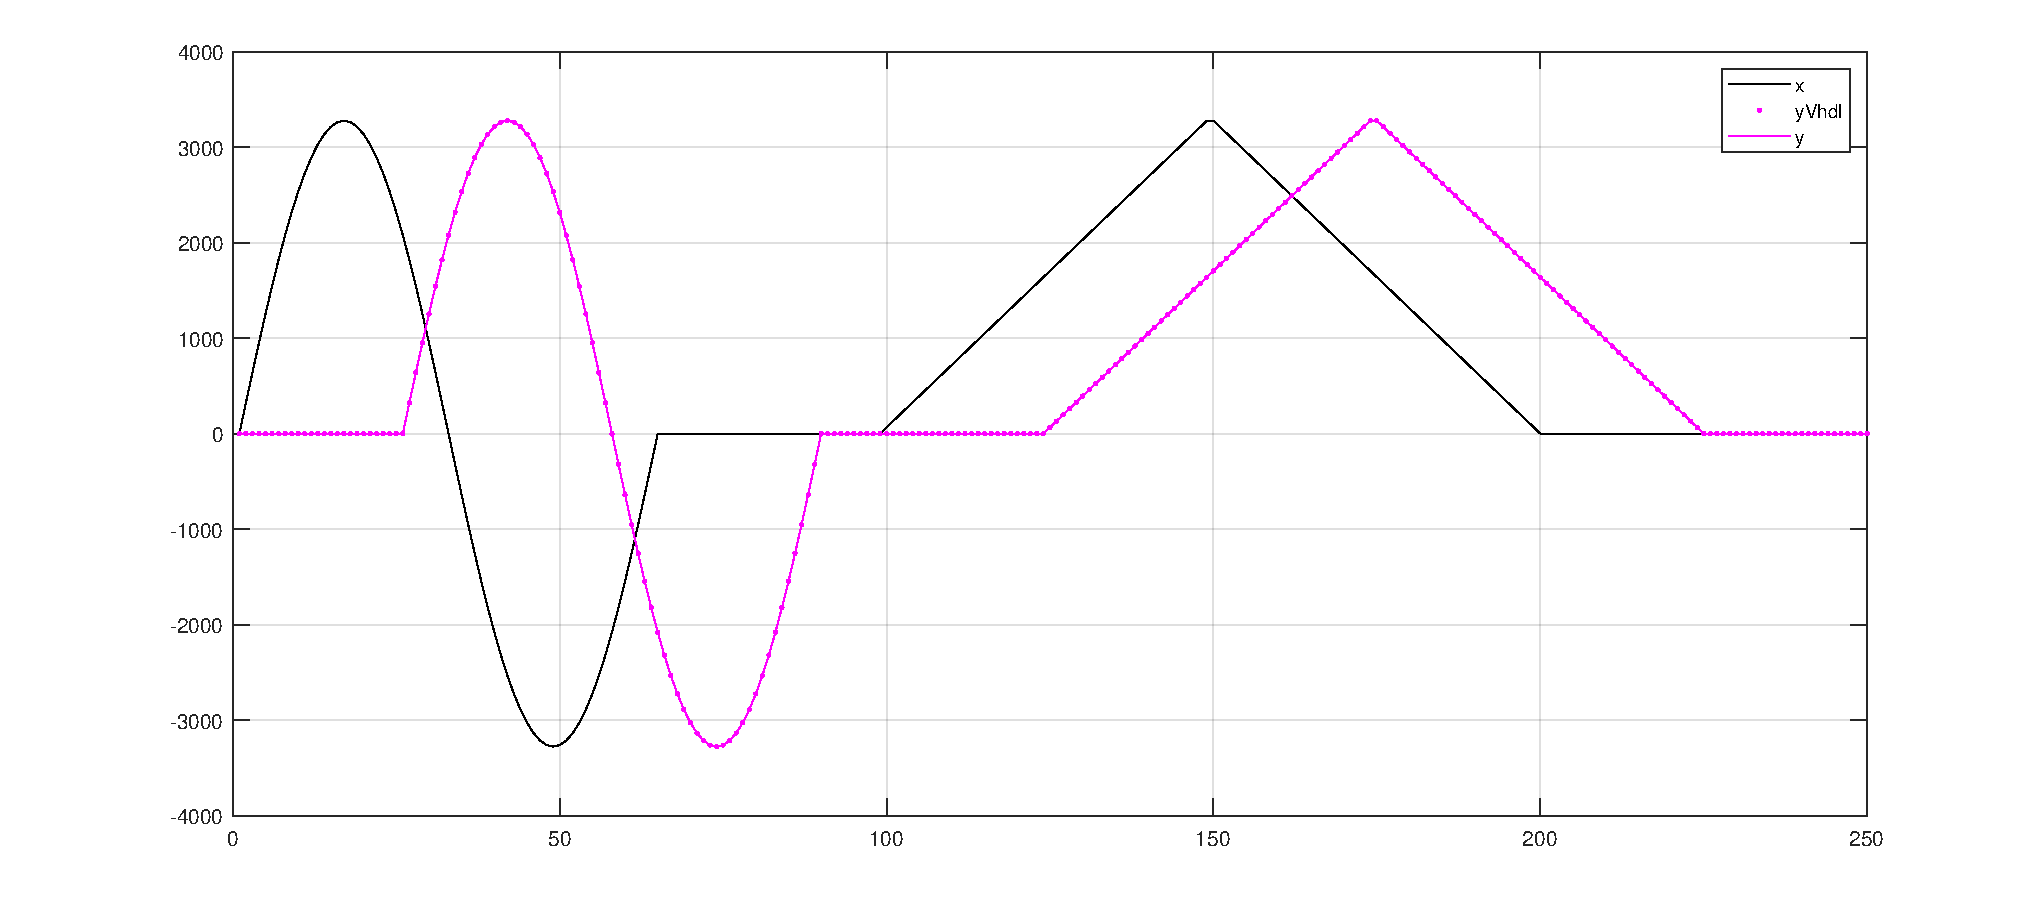
\includegraphics[width=0.9\textwidth]{papers/fpga/images/output.pdf}
	\caption{Output \label{fpga:fig:output}}
\end{figure}

Figure \ref{fpga:fig:output} shows the final result of the whole pipeline, As expected the signal is the same but delayed by the time the processing needed. 
\begin{figure}[h]
	\centering
	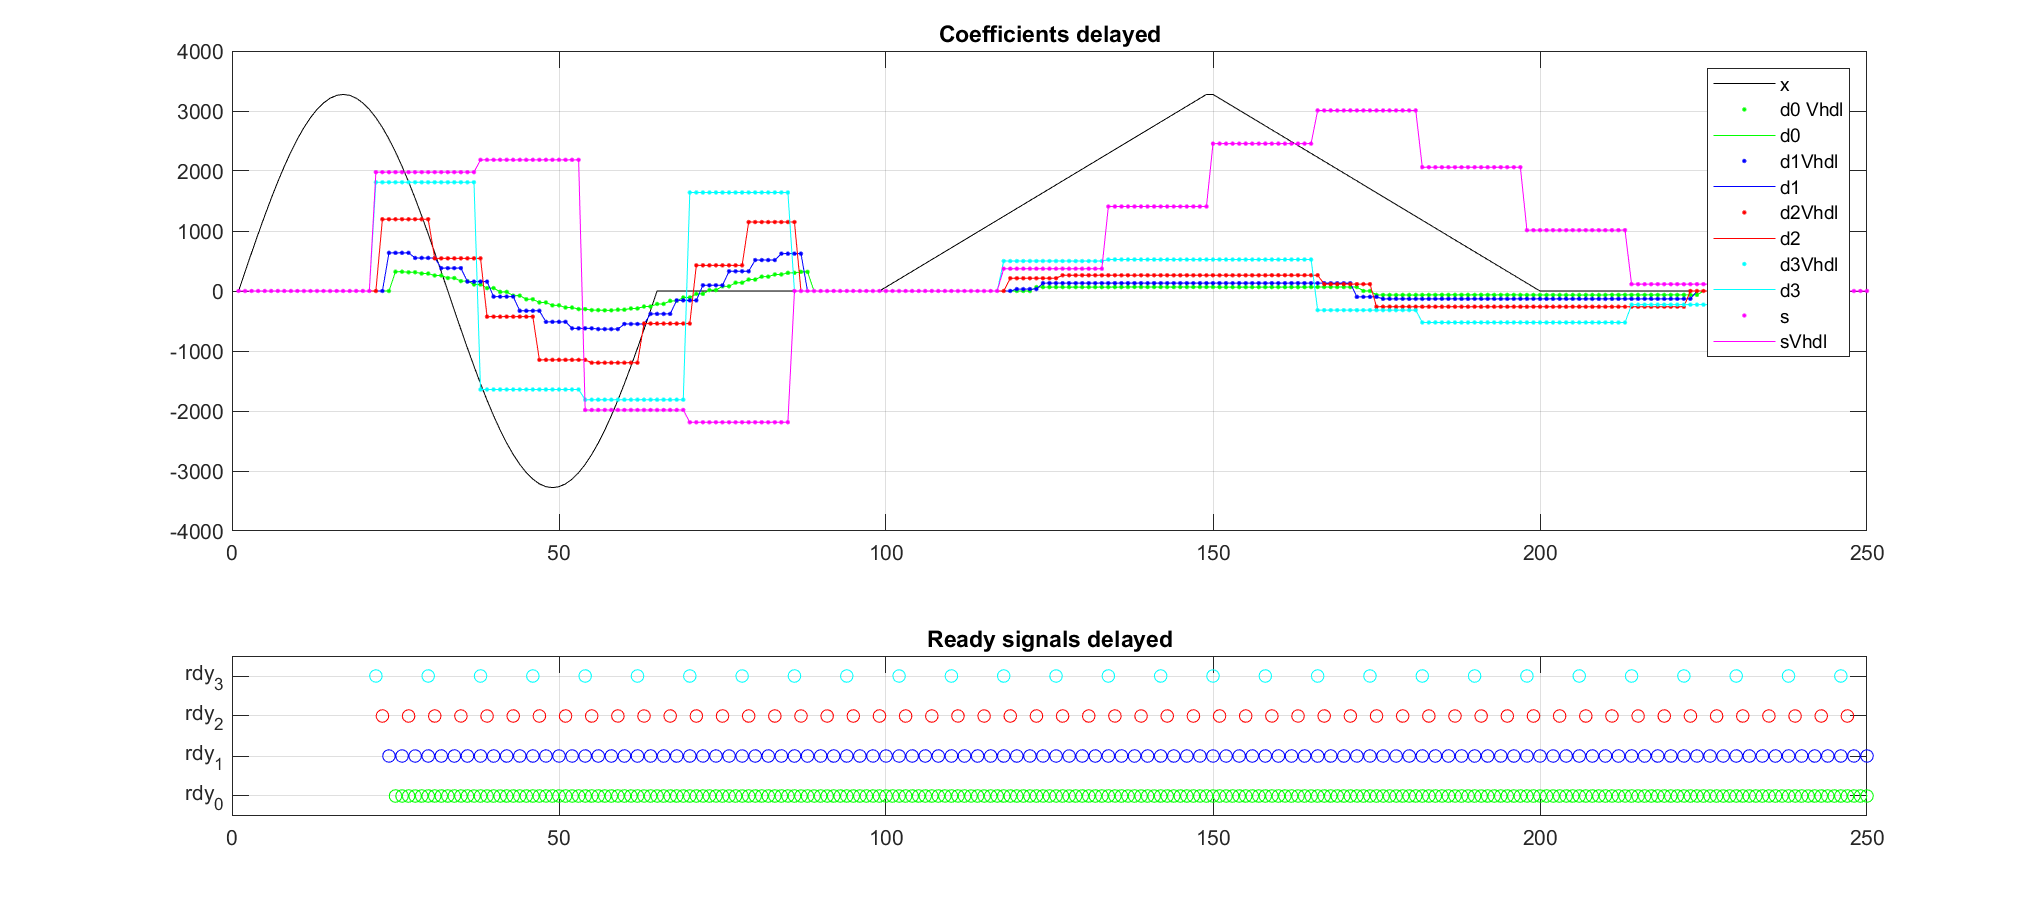
\includegraphics[width=0.9\textwidth]{papers/fpga/images/coefs_delayed.pdf}
	\caption{Coefficients and ready signals after delaying \label{fpga:fig:coeff_delayed}}
\end{figure}

Also interesting is how the coefficients and signals look inside the simulation (figure \ref{fpga:fig:coefficients}). 
In a screenshot the coefficients of all recursive steps are visible. 
There is clearly visible, that the signal losses information in de deeper stages. 
This is because every step the detail information (higher frequencies) get subtracted and only the low frequencies stay.

\begin{figure}[h]
	\centering
	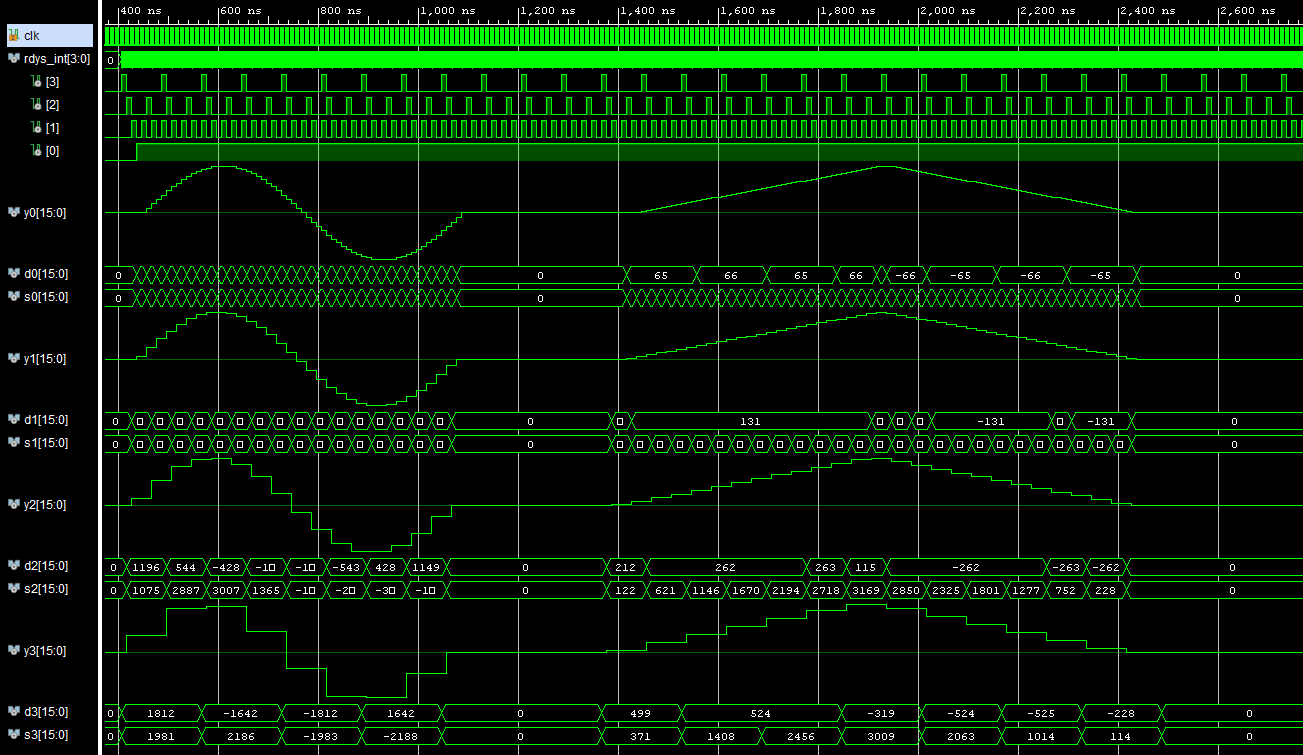
\includegraphics[width=0.9\textwidth]{papers/fpga/images/inv_branching_screenshot.PNG}
	\caption{Coefficients in simulation \label{fpga:fig:sim}}
\end{figure}

\newpage

%The idea is to have a data stream \texttt{x} an a ready \texttt{rdy} signal. The ready signal indicates when the input from the data stream is valid. The input is only read and processed if the ready signal is high. Then we build a block which contains the signal processing which was presented in section \ref{fpga:polyphase}. The Block then throws out the wavelet coefficients and also the ready signal for further processing. In a next stage a block for inverse transformation is used to recover the input signal.
%In this block we then implement the Wavelet Transformation with, in our case, the Haar Wavelet. Another goal was to create a structure to implement different wavelet transformations later. In this way of implementation  it should be possible to implement transformations with different wavelets in the same block (Picture \ref{fpga:haar_inv_haar}). 
%
%\begin{figure}[h]
%	\includegraphics[width=0.49\textwidth]{images/haar.pdf}
%	\includegraphics[width=0.49\textwidth]{images/inv_haar.pdf}
%	\caption{Haar und inverse Haar transformation \label{fpga:haar_inv_haar}}
%\end{figure}

%\begin{figure}[h!]
%	\centering
%	\begin{subfigure}[b]{\linewidth}
%		\centering
%		\includegraphics[width=0.49\textwidth]{images/haar.pdf}
%		\caption{Haar}
%	\end{subfigure}
%	\begin{subfigure}[b]{\linewidth}
%		\centering
%		\includegraphics[width=0.49\textwidth]{images/inv_haar.pdf}
%		\caption{Inverse haar}
%	\end{subfigure}
%	\caption{Haar and inverse Haar transformation \label{fpga:haar_inv_haar}}
%\end{figure}

%In this picture it is also visible that for every two input samples we get two wavelet coefficients. This corresponds to the sub sampling into two streams. The ready signal gets also delayed to match the speed of the output coefficients. In the inverse Haar block the coefficients get reconstructed to the original input stream.







\section{Conclusion}
\rhead{Conclusion}

In our view this project was a success. We were able to use some of the knowledge gained in this course to implement a hardware version of a wavelet transformation.

All Codes (VHDL, MATLAB) are stored in the github repository belonging to this book. \cite{fpga:gitrepo-wavelets}

The frequency selectivity of the Haar wavelet is low and not suitalbe for audio applications.
An change of gain of a coefficient would result in various distortions to the output signal.

\printbibliography[heading=subbibliography]
\end{refsection}
